\chapter{Evaluation}
In order to evaluate the effectiveness of CRAFTS' prediction methods, we run each method on the workloads outlined in \Cref{ch:workloads}. At the beginning of each experiment, the tuner is run on the baseline workload to tune the parameters of the prediction algorithm. This is done to ensure that the tuning is done with minimal anomalies present. Tuning in this way allows us to see how the various algorithms respond to anomalies after an extended period of ``regular'' traffic.

Each predictor will attempt to predict traffic for the week of October 14th in each workload and can use how ever much data it needs before that time for training. The effectiveness of each algorithm is measured using root mean squared deviation (RMSD), as discussed in \Cref{eq:rmsd}. We further break the results down into over-estimations and under-estimations, giving the RMSD for each as well as the percent of predictions which fell into each category. This is done because, in a real-world environment, under-estimations are more costly than over-estimations and we would favor predictors which are more likely to over-estimate than under-estimate. In workloads which contain anomalies, we analyze how the predictor performs during the anomaly separately from how it performs during normal traffic. This allows us to get a more complete view of how a predictor handles anomalies.

In the baseline workload, the goal is to minimize the RMSD for all types. The same is true for regular traffic in all anomalous workloads. For the anomalous training workloads, the predictor should ideally minimize RMSD of all types as well. This result would mean that the anomaly in the training data did not affect the future predictions. In the outage horizon workload, we want to see 100\% over-estimation and maximize over-estimation RMSD during this time. This means that the predictor has successfully ignored the outage. Inversely, we want to see 100\% underestimation and maximize under-estimation RMSD for the spike training workload. These values indicate that the spike was successfully ignored.

The following sections include the evaluation results for each predictor and an analysis of those results. In the graphs below, the light blue line represents the observed data and the black line shows our own predictions.

\section{Translation}
Results for regular traffic show that the translation predictor is prone to underestimation. This is likely due to fluctuations in week by week traffic or a linear trend in the data. In the case of the latter, translation would not be able to account for this since it has no mechanism to account for trends of any kind.

Training data anomalies seriously impact the effectiveness of translation. Since the translation predictor makes no attempt to account for any sort of anomalies, these anomalies are simply preserved and translated into the prediction horizon.

As one would expect, translation is very tolerant to anomalies in the prediction horizon. Since translation makes a long-term prediction, these anomalies won't have an effect on this predictors results until they are part of the training data the next week.

\begin{figure}
\centering
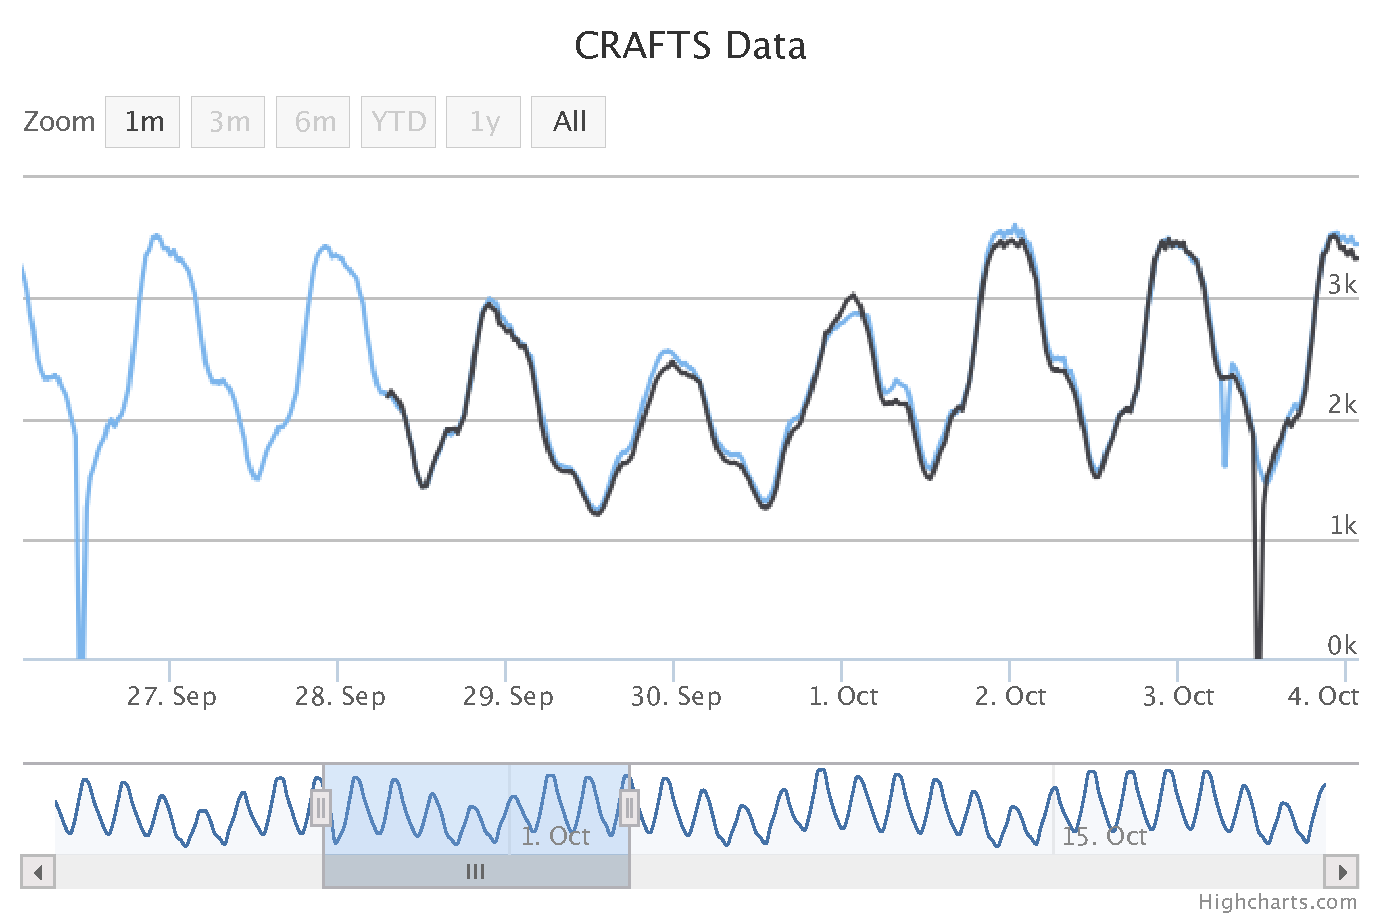
\includegraphics[width=\textwidth]{results/graphs/translation_outage.pdf}
\caption{An outage translated by the translation predictor}
\label{fig:translation_outage}
\end{figure}

\begin{figure}
\centering
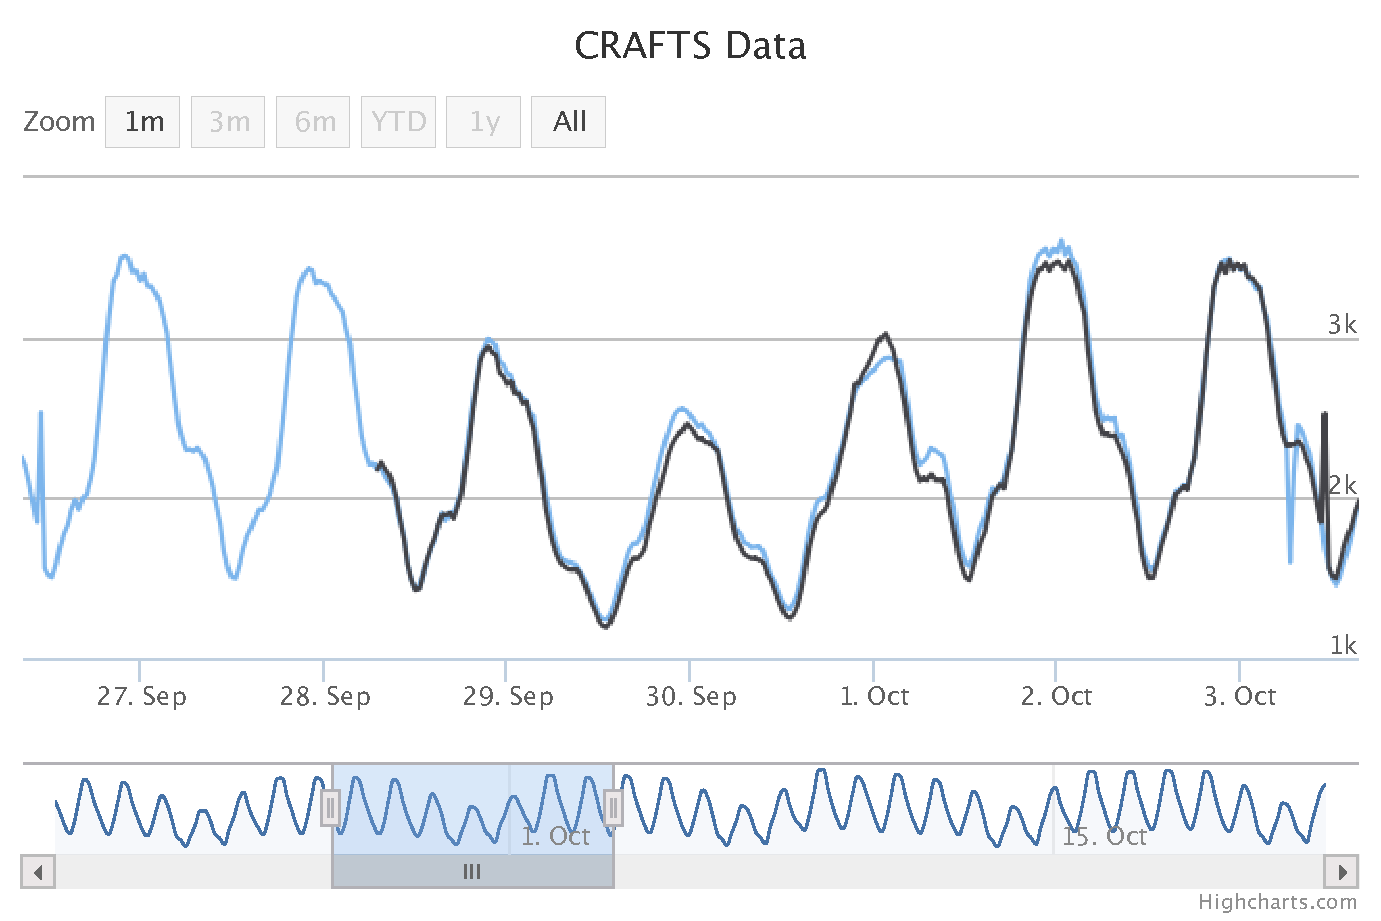
\includegraphics[width=\textwidth]{results/graphs/translation_spike.pdf}
\caption{A usage spike translated by the translation predictor}
\label{fig:translation_spike}
\end{figure}

\begin{table}[H]
\centering
\begin{tabular}{| l | l | l |}
\hline
Type & RMSD & Percent \\ \hline
Under & 113 & 68.7\% \\ \hline
Over & 76 & 31.3\% \\ \hline
Total & 103 & \\ \hline
\end{tabular}
\caption{Translation predictor results for the baseline workload}
\end{table}

% Outage workloads

\begin{table}[H]
\centering
\begin{tabular}{| l | l | l |}
\hline
Type & RMSD & Percent \\ \hline
Under & 122 & 68.7\% \\ \hline
Over & 76 & 31.3\% \\ \hline
Total & 110 & \\ \hline
\end{tabular}
\caption{Translation predictor results for the 10-minute outage workload}
\end{table}

\begin{table}[H]
\centering
\begin{tabular}{| l | l | l |}
\hline
Type & RMSD & Percent \\ \hline
Under & 132 & 68.8\% \\ \hline
Over & 76 & 31.2\% \\ \hline
Total & 117 & \\ \hline
\end{tabular}
\caption{Translation predictor results for the 30-minute outage workload}
\end{table}

\begin{table}[H]
\centering
\begin{tabular}{| l | l | l |}
\hline
Type & RMSD & Percent \\ \hline
Under & 145 & 68.9\% \\ \hline
Over & 76 & 31.1\% \\ \hline
Total & 127 & \\ \hline
\end{tabular}
\caption{Translation predictor results for the 60-minute outage workload}
\end{table}

% Spike workloads

\begin{table}[H]
\centering
\begin{tabular}{| l | l | l |}
\hline
Type & RMSD & Percent \\ \hline
Under & 113 & 68.7\% \\ \hline
Over & 83 & 31.3\% \\ \hline
Total & 105 & \\ \hline
\end{tabular}
\caption{predictor results for the low spike workload}
\end{table}

\begin{table}[H]
\centering
\begin{tabular}{| l | l | l |}
\hline
Type & RMSD & Percent \\ \hline
Under & 113 & 68.7\% \\ \hline
Over & 91 & 31.3\% \\ \hline
Total & 107 & \\ \hline
\end{tabular}
\caption{predictor results for the mid spike workload}
\end{table}

\begin{table}[H]
\centering
\begin{tabular}{| l | l | l |}
\hline
Type & RMSD & Percent \\ \hline
Under & 113 & 68.7\% \\ \hline
Over & 102 & 31.3\% \\ \hline
Total & 110 & \\ \hline
\end{tabular}
\caption{predictor results for the high spike workload}
\end{table}

\section{Fast Fourier Transform}
With an optimized smoothing percentage of 96\%, the FFT predictor performs slightly worse than the translation predictor for regular traffic, but sees a 40\% decrease in error for the training outage and an 87\% decrease in error for the training spike workload. While this is a large improvement, the amount of error we observed for the training anomalies was still higher than expected. In order to further investigate these results, we ran a second evaluation on the training outage workload, this time with 99\% filtering. This time we observed a 58\% decrease in error within the anomaly space over the 96\% smoothing run. We also observed a slight decrease in error for regular traffic as well.

In this case, it seems that the tuner did not perform as we had hoped it to. Since there were no anomalies in the data which the \textsf{tuner} was run on, the optimal smoothing percentage was calculated without being able to take these kinds of anomalies into account. Further analysis of the deficiencies in our \textsf{tuner} implementation can be seen in \Cref{ch:conclusions}.

Similarly to the translation predictor, FFT makes long term decisions, so its predictions are unaffected by anomalies in the prediction horizon.

\begin{table}[H]
\centering
\begin{tabular}{| l | l | l |}
\hline
Type & RMSD & Percent \\ \hline
Under & 140 & 76.2\% \\ \hline
Over & 61 & 23.8\% \\ \hline
Total & 125 & \\ \hline
\end{tabular}
\caption{FFT predictor results for the baseline workload}
\end{table}

\begin{figure}[H]
\centering
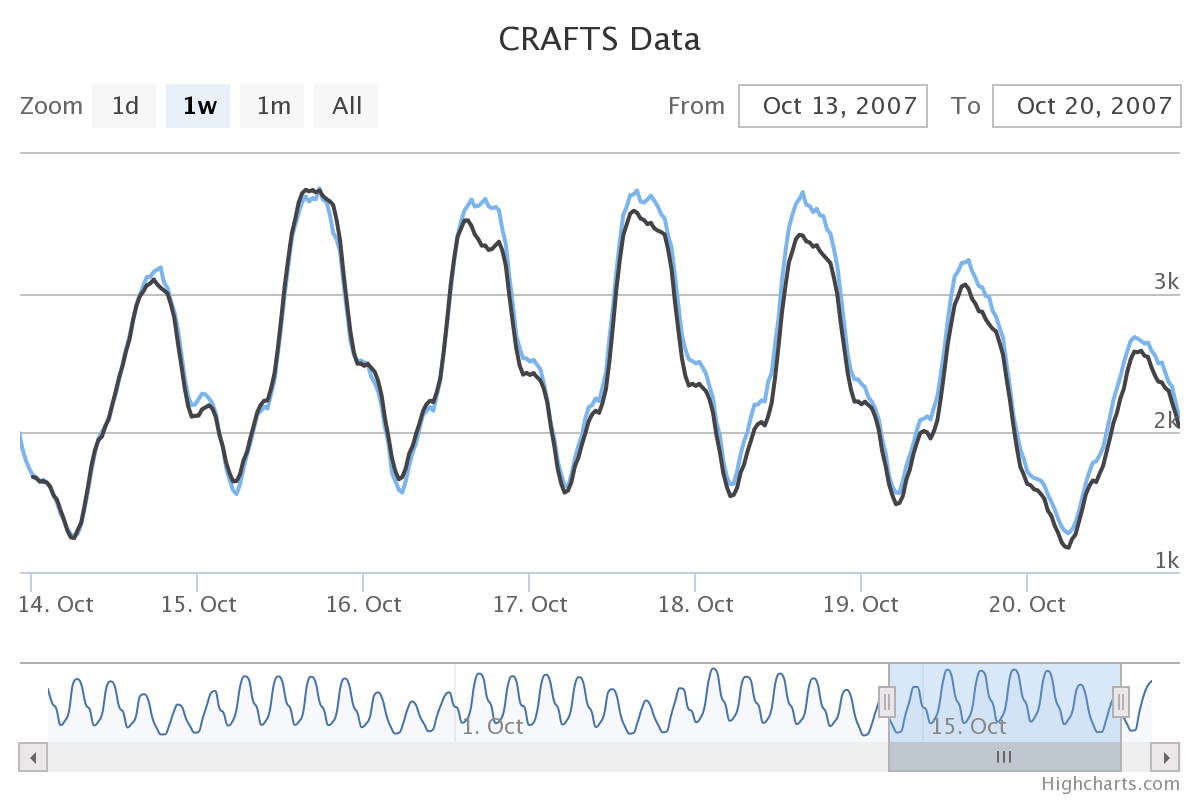
\includegraphics[width=\textwidth]{results/graphs/fft_baseline.png}
\caption{FFT prediction results for the baseline workload}
\label{fig:fft_b}
\end{figure}

\begin{table}[H]
\centering
\begin{tabular}{| l | l | l | l | l |}
\hline
Type & \multicolumn{2}{c |}{Regular} & \multicolumn{2}{c |}{Anomalous} \\ \hline
 & RMSD & Percent & RMSD & Percent \\ \hline
Under & 211 & 74.1\% & 1741 & 100.0\% \\ \hline
Over & 85 & 25.9\% & 0 & 0.0\% \\ \hline
Total & 186 & & 1741 & \\ \hline
\end{tabular}
\caption{FFT predictor results for the training outage workload with 96\% filtering}
\end{table}

\begin{figure}[H]
\centering
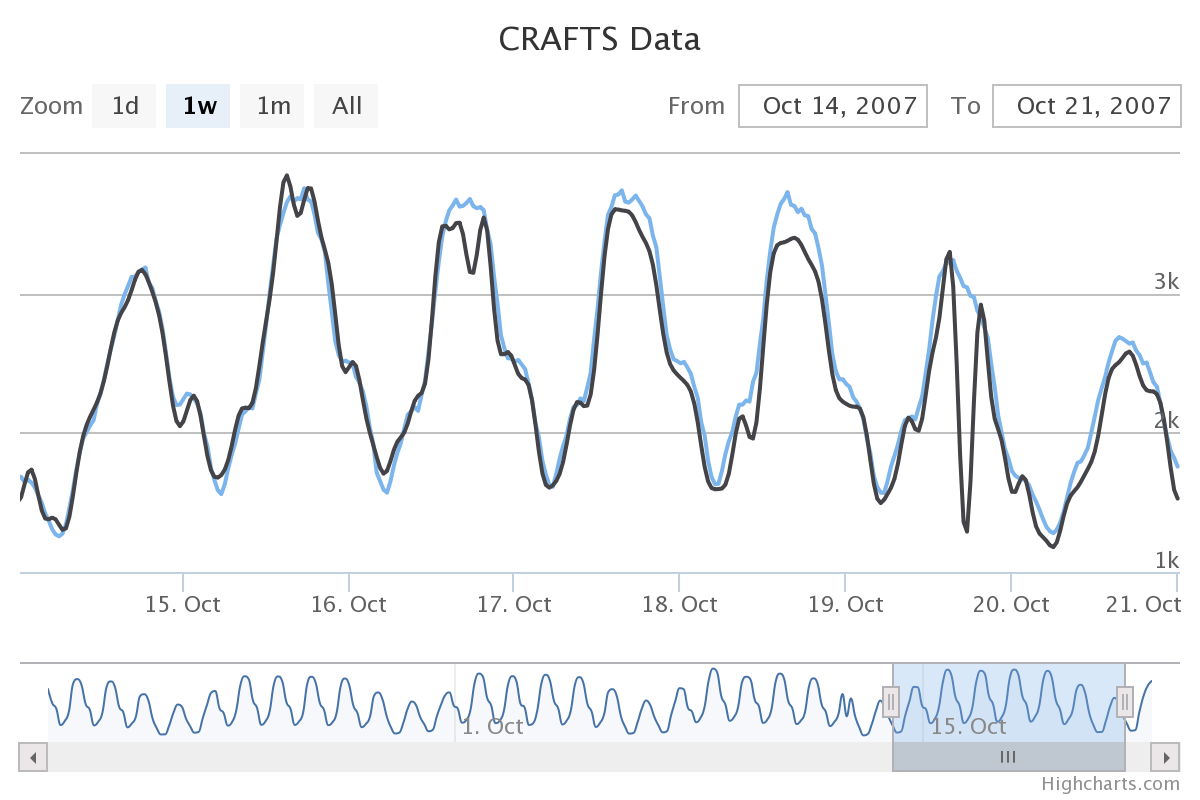
\includegraphics[width=\textwidth]{results/graphs/fft_training_outage_96.png}
\caption{FFT prediction results for the training outage workload with 96\% filtering}
\label{fig:fft_to96}
\end{figure}

\begin{table}[H]
\centering
\begin{tabular}{| l | l | l | l | l |}
\hline
Type & \multicolumn{2}{c |}{Regular} & \multicolumn{2}{c |}{Anomalous} \\ \hline
 & RMSD & Percent & RMSD & Percent \\ \hline
Under & 195 & 75.0\% & 721 & 100.0\% \\ \hline
Over & 88 & 25.0\% & 0 & 0.0\% \\ \hline
Total & 175 & & 721 & \\ \hline
\end{tabular}
\caption{FFT predictor results for the training outage workload with 99\% filtering}
\end{table}

\begin{figure}[H]
\centering
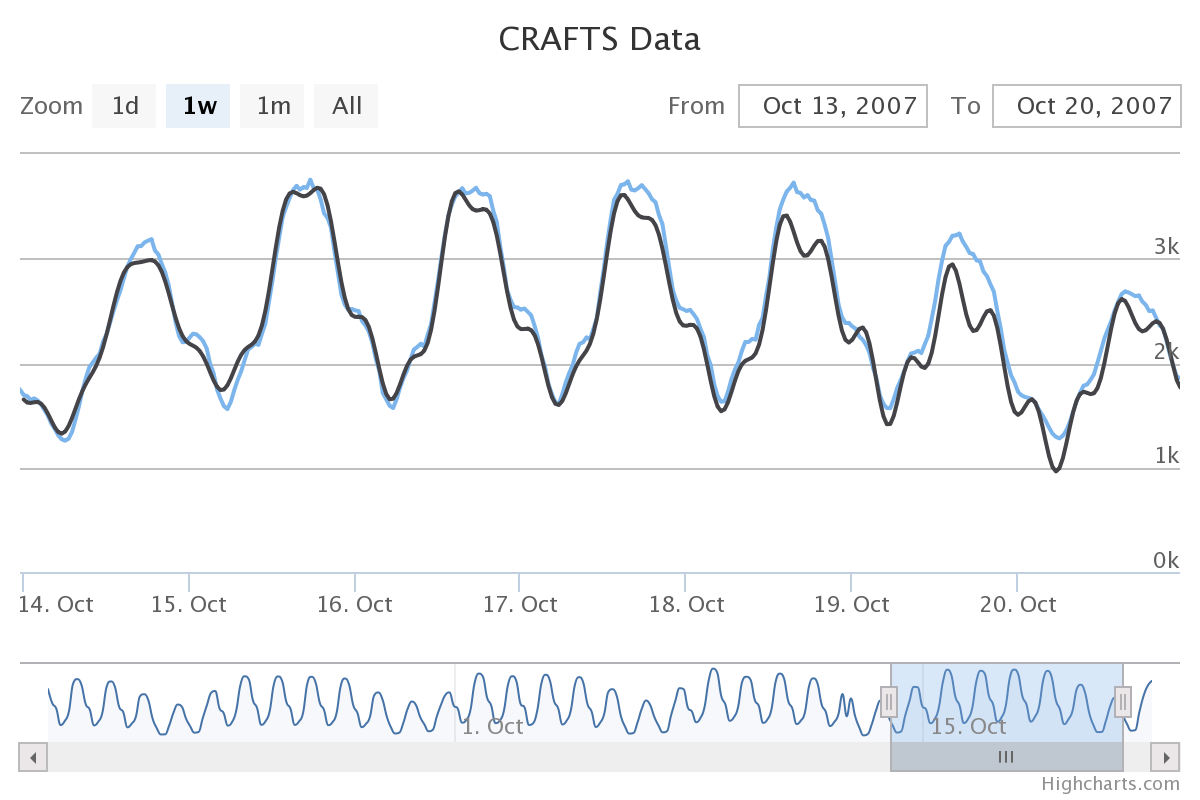
\includegraphics[width=\textwidth]{results/graphs/fft_training_outage_99.png}
\caption{FFT prediction results for the training outage workload with 99\% filtering}
\label{fig:fft_to99}
\end{figure}

\begin{table}[H]
\centering
\begin{tabular}{| l | l | l | l | l |}
\hline
Type & \multicolumn{2}{c |}{Regular} & \multicolumn{2}{c |}{Anomalous} \\ \hline
 & RMSD & Percent & RMSD & Percent \\ \hline
Under & 139 & 75.9\% & 0 & 0.0\% \\ \hline
Over & 194 & 24.1\% & 2869 & 100.0\% \\ \hline
Total & 154 & & 2869 & \\ \hline
\end{tabular}
\caption{FFT predictor results for the horizon outage workload}
\end{table}

\begin{figure}[H]
\centering
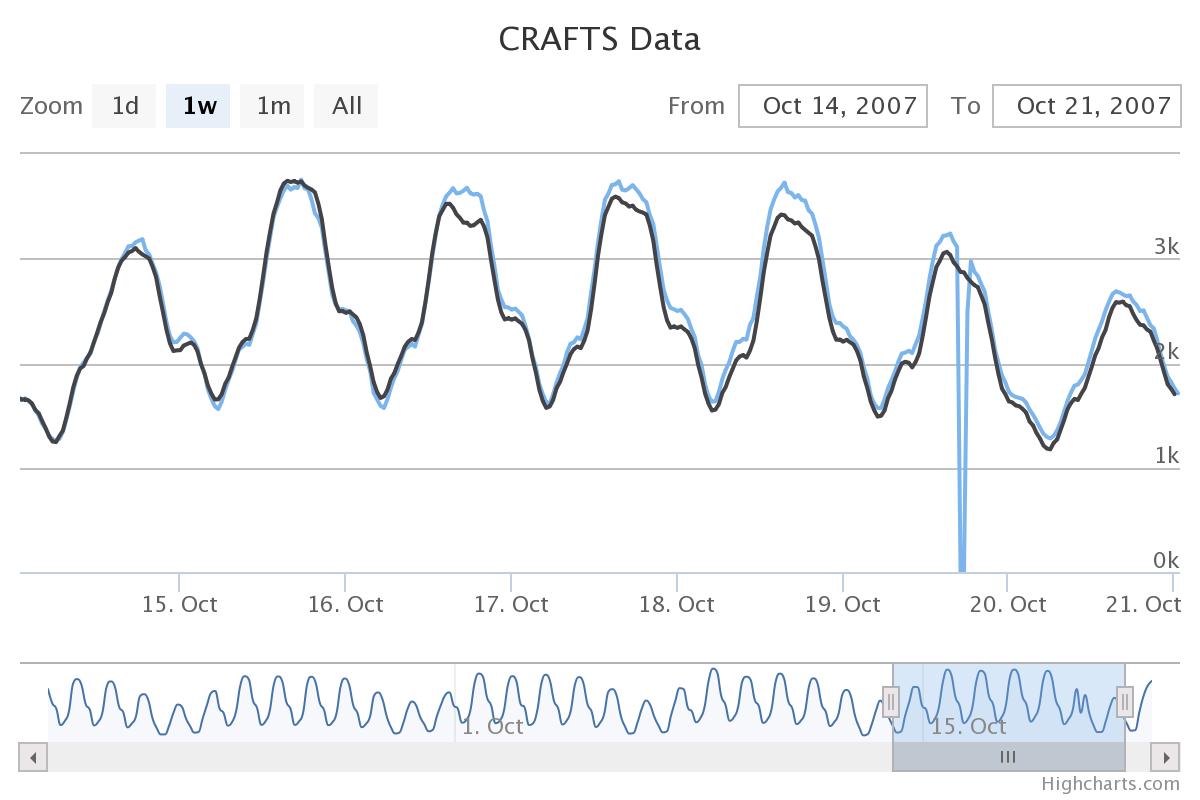
\includegraphics[width=\textwidth]{results/graphs/fft_horizon_outage.png}
\caption{FFT prediction results for the horizon outage workload}
\label{fig:fft_ho}
\end{figure}

\begin{table}[H]
\centering
\begin{tabular}{| l | l | l | l | l |}
\hline
Type & \multicolumn{2}{c |}{Regular} & \multicolumn{2}{c |}{Anomalous} \\ \hline
 & RMSD & Percent & RMSD & Percent \\ \hline
Under & 143 & 74.6\% & 0 & 0.0\% \\ \hline
Over & 86 & 25.4\% & 427 & 100.0\% \\ \hline
Total & 131 & & 427 & \\ \hline
\end{tabular}
\caption{FFT predictor results for the training spike workload}
\end{table}

\begin{figure}[H]
\centering
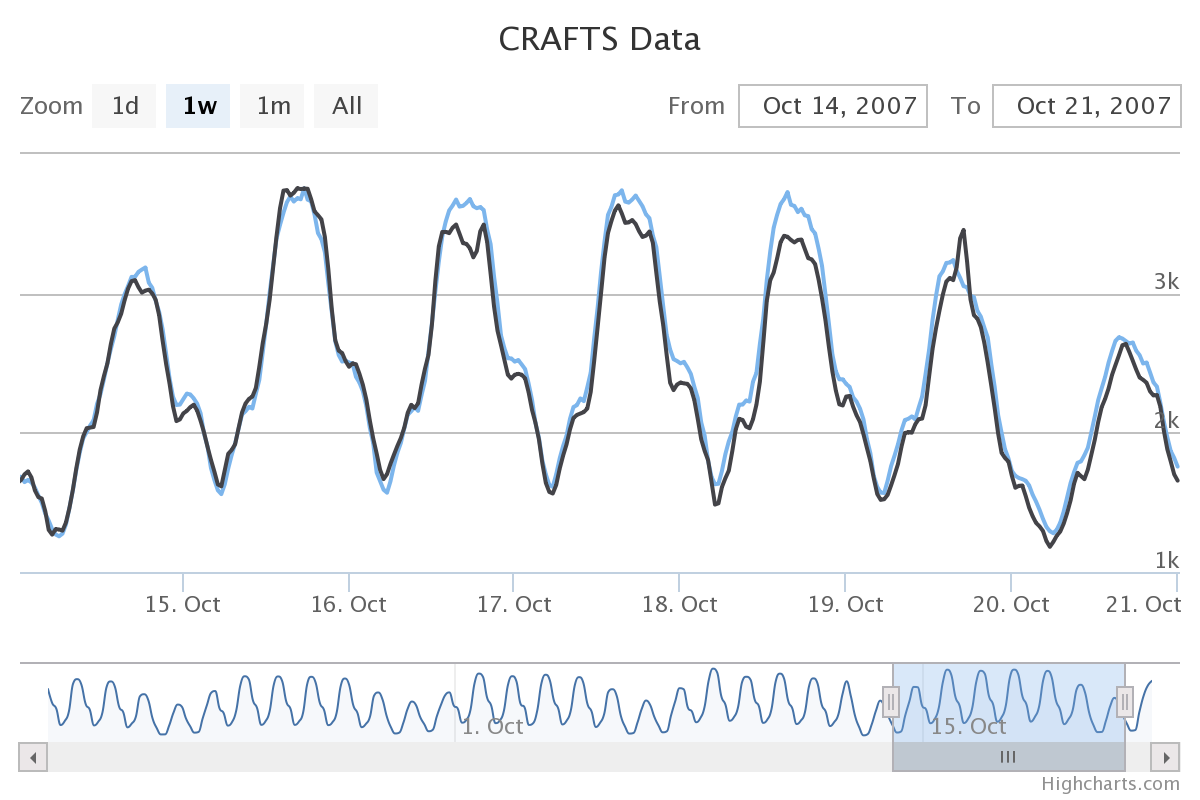
\includegraphics[width=\textwidth]{results/graphs/fft_training_spike.png}
\caption{FFT prediction results for the training spike workload}
\label{fig:fft_ts}
\end{figure}

\begin{table}[H]
\centering
\begin{tabular}{| l | l | l | l | l |}
\hline
Type & \multicolumn{2}{c |}{Regular} & \multicolumn{2}{c |}{Anomalous} \\ \hline
 & RMSD & Percent & RMSD & Percent \\ \hline
Under & 181 & 76.1\% & 3239 & 100.0\% \\ \hline
Over & 61 & 23.9\% & 0 & 0.0\% \\ \hline
Total & 161 & & 3239 & \\ \hline
\end{tabular}
\caption{FFT predictor results for the horizon spike workload}
\end{table}

\begin{figure}[H]
\centering
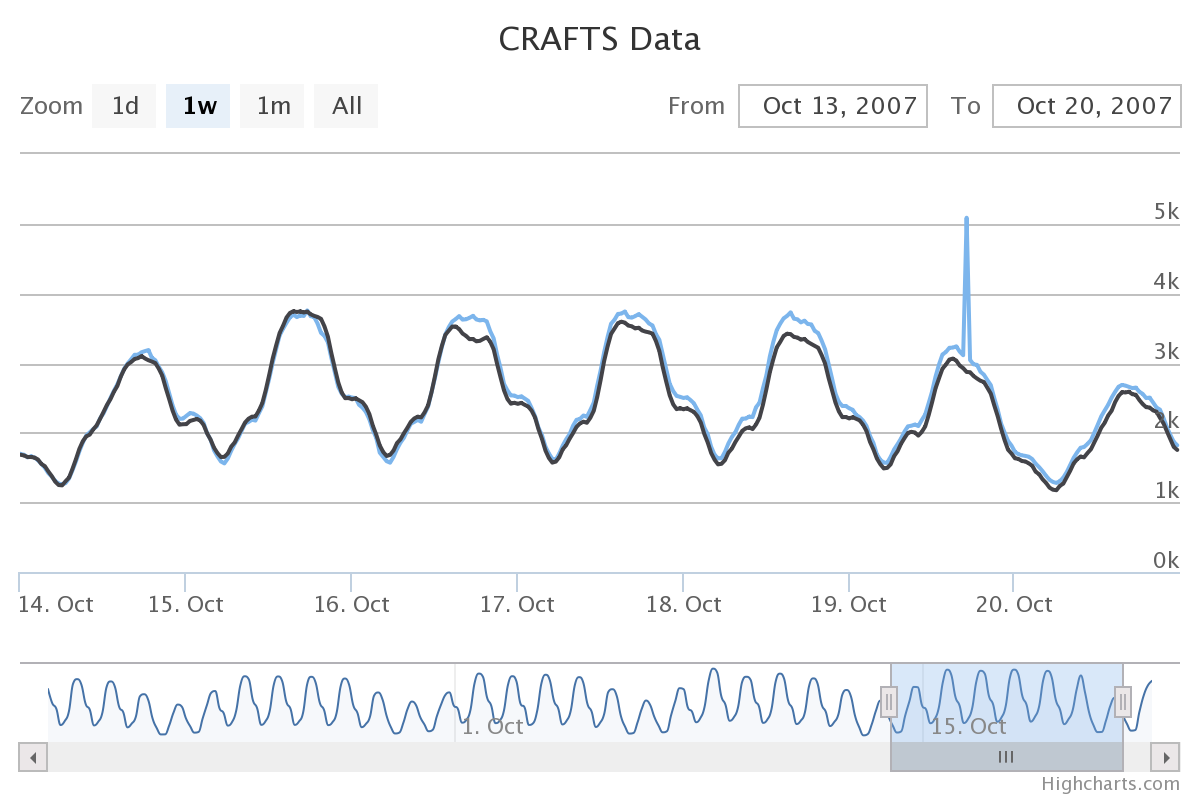
\includegraphics[width=\textwidth]{results/graphs/fft_horizon_spike.png}
\caption{FFT prediction results for the horizon spike workload}
\label{fig:fft_hs}
\end{figure}

\section{Linear Regression}
Linear regression performs neck and neck with the translation baseline for regular traffic, but truly shines when presented with training anomalies. Since the Thiel-Sen estimator is tolerant to outliers, the anomalies present in the training data are largely ignored. We observe RMSD values within the anomaly space smaller than any predictor evaluated thus far.

Again, as a long-term predictor, anomalies in the prediction horizon have no effect on the linear regression predictor's effectiveness.

\begin{table}[H]
\centering
\begin{tabular}{| l | l | l |}
\hline
Type & RMSD & Percent \\ \hline
Under & 138 & 89.2\% \\ \hline
Over & 32 & 10.8\% \\ \hline
Total & 131 & \\ \hline
\end{tabular}
\caption{Regression predictor results for the baseline workload}
\end{table}

\begin{figure}[H]
\centering
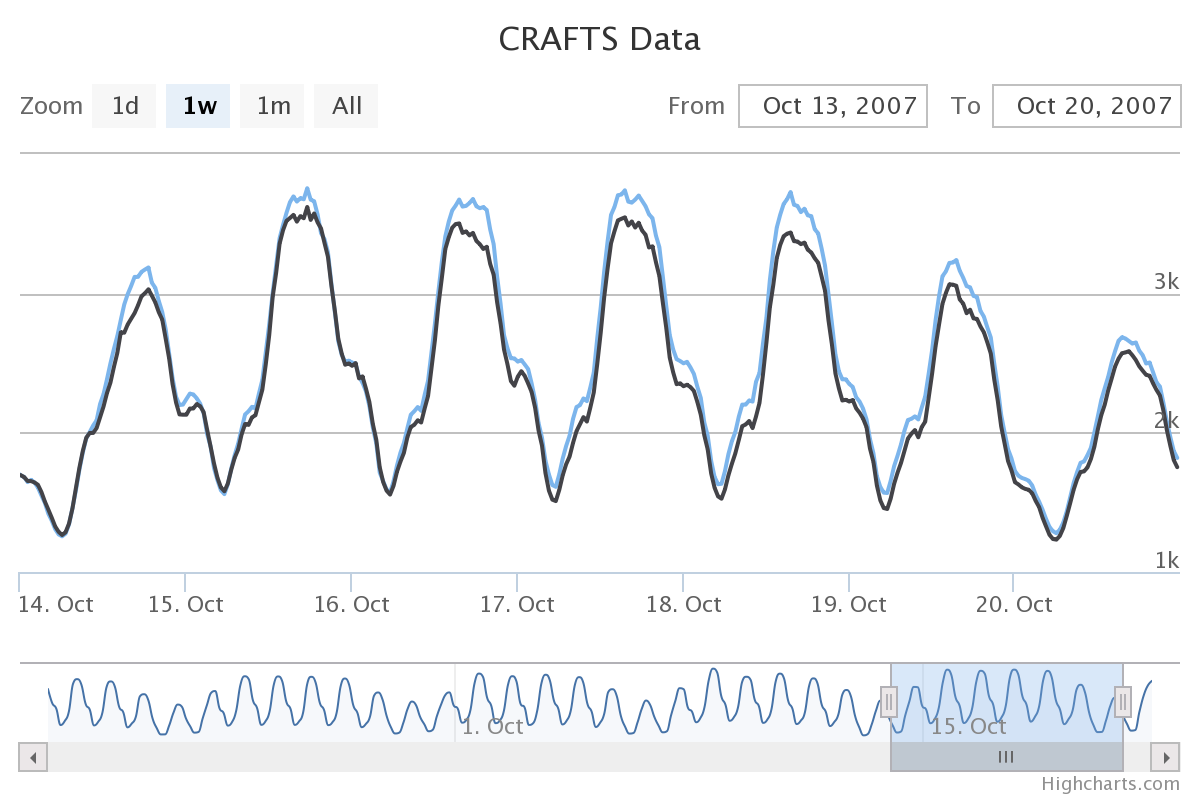
\includegraphics[width=\textwidth]{results/graphs/regression_baseline.png}
\caption{Regression prediction results for the baseline workload}
\label{fig:regression_b}
\end{figure}

\begin{table}[H]
\centering
\begin{tabular}{| l | l | l | l | l |}
\hline
Type & \multicolumn{2}{c |}{Regular} & \multicolumn{2}{c |}{Anomalous} \\ \hline
 & RMSD & Percent & RMSD & Percent \\ \hline
Under & 138 & 89.1\% & 270 & 100.0\% \\ \hline
Over & 32 & 10.9\% & 0 & 0.0\% \\ \hline
Total & 131 & & 270 & \\ \hline
\end{tabular}
\caption{Regression predictor results for the training outage workload}
\end{table}

\begin{figure}[H]
\centering
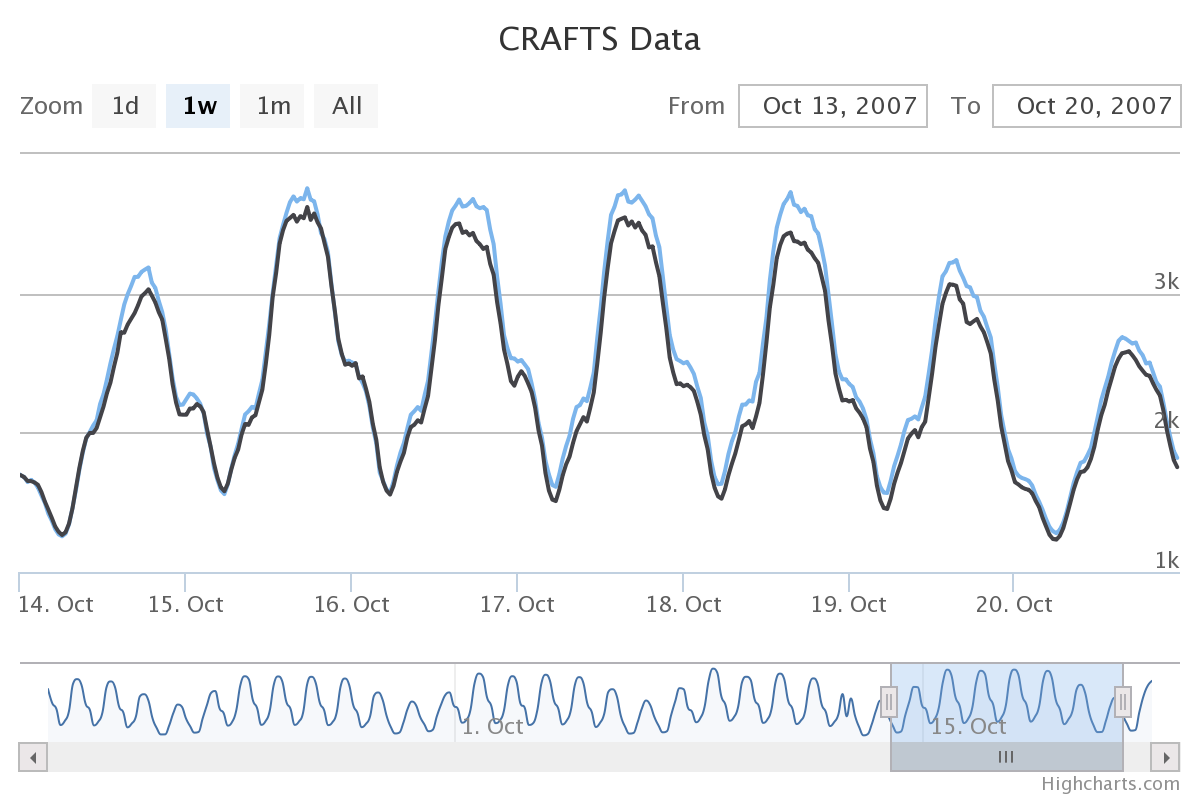
\includegraphics[width=\textwidth]{results/graphs/regression_training_outage.png}
\caption{Regression prediction results for the training outage workload}
\label{fig:regression_to}
\end{figure}

\begin{table}[H]
\centering
\begin{tabular}{| l | l | l | l | l |}
\hline
Type & \multicolumn{2}{c |}{Regular} & \multicolumn{2}{c |}{Anomalous} \\ \hline
 & RMSD & Percent & RMSD & Percent \\ \hline
Under & 138 & 89.0\% & 0 & 0.0\% \\ \hline
Over & 274 & 11.0\% & 2869 & 100.0\% \\ \hline
Total & 159 & & 2869 & \\ \hline
\end{tabular}
\caption{Regression predictor results for the horizon outage workload}
\end{table}

\begin{figure}[H]
\centering
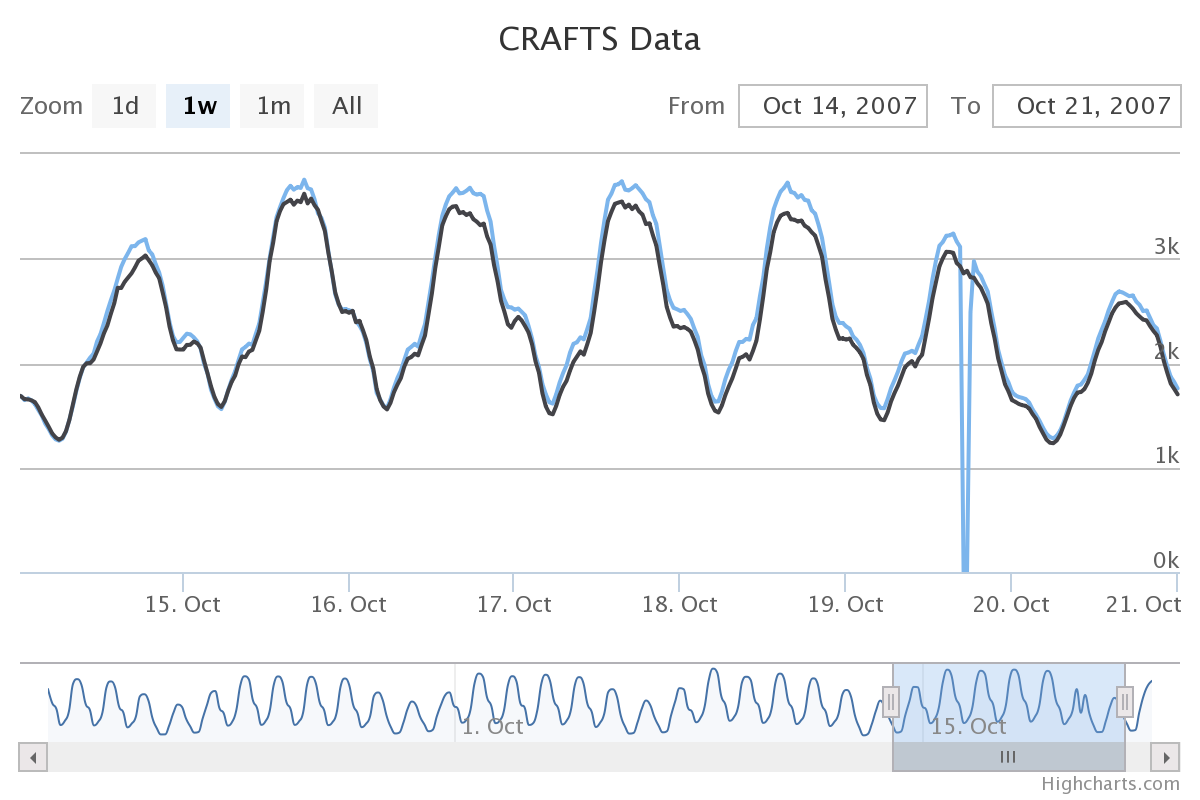
\includegraphics[width=\textwidth]{results/graphs/regression_horizon_outage.png}
\caption{Regression prediction results for the horizon outage workload}
\label{fig:regression_ho}
\end{figure}

\begin{table}[H]
\centering
\begin{tabular}{| l | l | l | l | l |}
\hline
Type & \multicolumn{2}{c |}{Regular} & \multicolumn{2}{c |}{Anomalous} \\ \hline
 & RMSD & Percent & RMSD & Percent \\ \hline
Under & 138 & 89.2\% & 177 & 100.0\% \\ \hline
Over & 32 & 10.8\% & 0 & 0.0\% \\ \hline
Total & 131 & & 177 & \\ \hline
\end{tabular}
\caption{Regression predictor results for the training spike workload}
\end{table}

\begin{figure}[H]
\centering
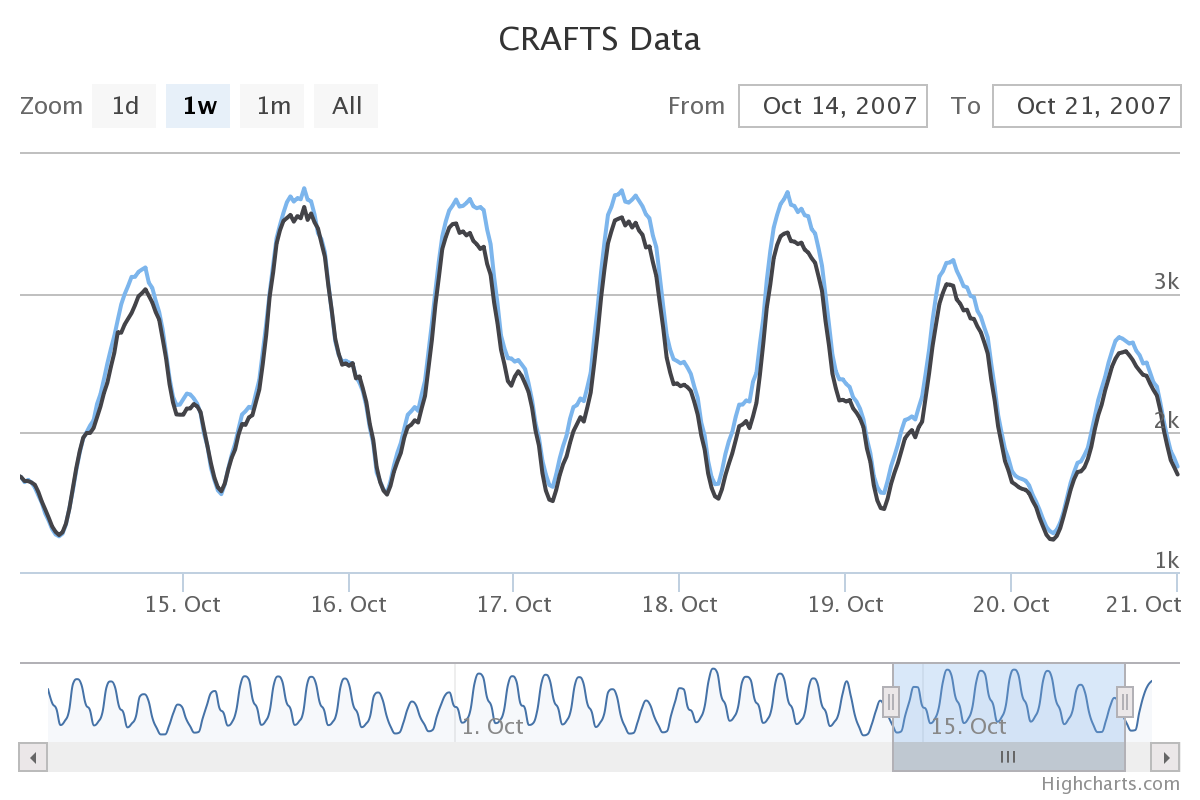
\includegraphics[width=\textwidth]{results/graphs/regression_training_spike.png}
\caption{Regression prediction results for the training spike workload}
\label{fig:regression_ts}
\end{figure}

\begin{table}[H]
\centering
\begin{tabular}{| l | l | l | l | l |}
\hline
Type & \multicolumn{2}{c |}{Regular} & \multicolumn{2}{c |}{Anomalous} \\ \hline
 & RMSD & Percent & RMSD & Percent \\ \hline
Under & 175 & 89.2\% & 3260 & 100.0\% \\ \hline
Over & 32 & 10.8\% & 0 & 0.0\% \\ \hline
Total & 166 & & 3260 & \\ \hline
\end{tabular}
\caption{Regression predictor results for the horizon spike workload}
\end{table}

\begin{figure}[H]
\centering
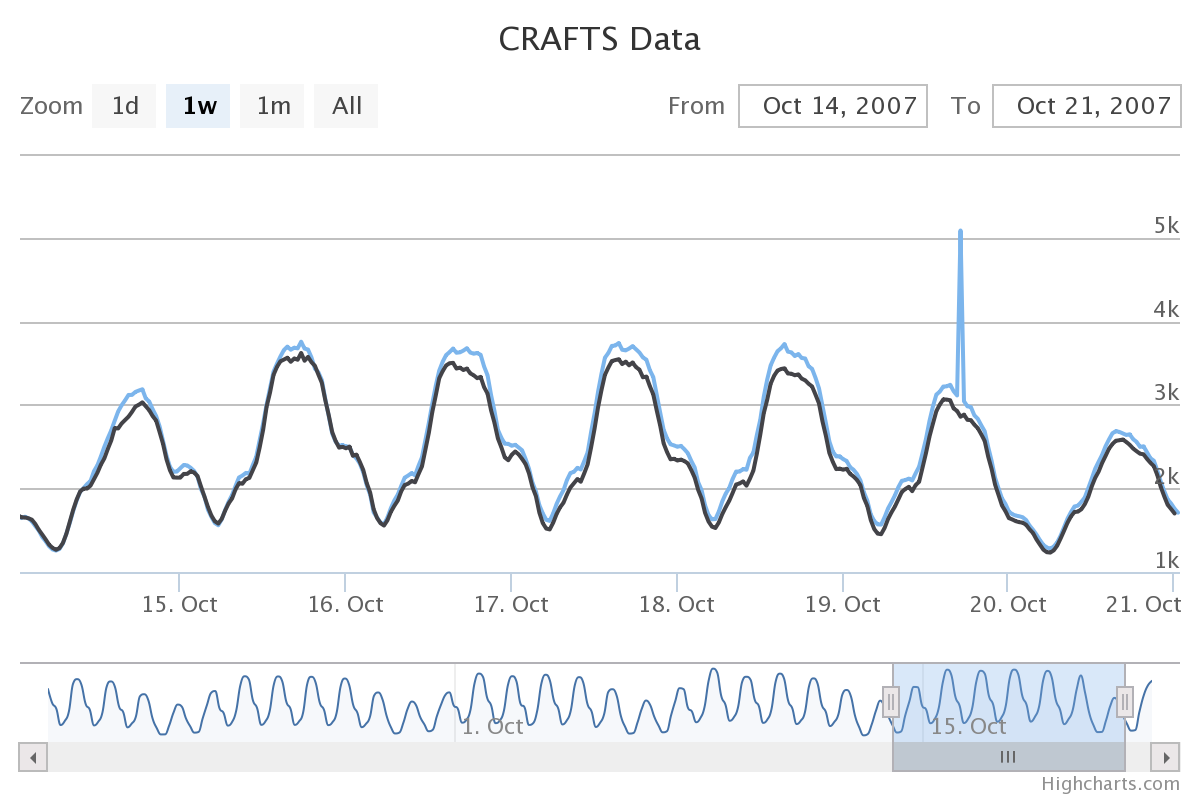
\includegraphics[width=\textwidth]{results/graphs/regression_horizon_spike.png}
\caption{Regression prediction results for the horizon spike workload}
\label{fig:regression_hs}
\end{figure}

\section{Discrete-Time Markov Chain}
The Markov predictor produced the best results for most regular traffic scenarios we have seen so far, but as seen in \Cref{fig:markov_b,fig:markov_ho,fig:markov_ts,fig:markov_hs}, there are some peculiar anomalies present in its predictions. These sudden dips can likely be attributed to the periodic nature of the data. Since the transition probability matrix is based on the likelihood of moving between one bucket and another bucket, a perfect sine wave would produce a transition probability matrix where it is equally likely to move to a higher bucket or a lower bucket. Similarly, since our data is periodic, it is likely that in some cases the probability of moving to a lower bucket is more likely than moving to a higher bucket, even if there is an upwards trend in the observations.

The Markov predictor is also very sensitive to anomalies in the prediction horizon. Since this predictor makes predictions only a short amount of time into the future, it is likely that a prediction will be made while an anomaly is occurring and be used as the base observation in the transition probability matrix.

The short-term nature of this predictor also has repercussions on the \textsf{planner's} ability to do its job properly. This will be discussed further in \Cref{ch:conclusions}.

\begin{table}[H]
\centering
\begin{tabular}{| l | l | l | l | l | l |}
\hline
Type & RMSD & Percent \\ \hline
Under & 27 & 74.0\% \\ \hline
Over & 22 & 26.0\% \\ \hline
Total & 26 & \\ \hline
\end{tabular}
\caption{Markov predictor results for the baseline workload}
\end{table}

% Outage workloads

\begin{table}[H]
\centering
\begin{tabular}{| l | l | l |}
\hline
Type & RMSD & Percent \\ \hline
Under & 52 & 80.8\% \\ \hline
Over & 39 & 19.2\% \\ \hline
Total & 50 & \\ \hline
\end{tabular}
\caption{predictor results for the 10-minute outage workload}
\end{table}

\begin{table}[H]
\centering
\begin{tabular}{| l | l | l |}
\hline
Type & RMSD & Percent \\ \hline
Under & 52 & 80.9\% \\ \hline
Over & 40 & 19.1\% \\ \hline
Total & 50 & \\ \hline
\end{tabular}
\caption{predictor results for the 30-minute outage workload}
\end{table}

\begin{table}[H]
\centering
\begin{tabular}{| l | l | l |}
\hline
Type & RMSD & Percent \\ \hline
Under & 52 & 80.9\% \\ \hline
Over & 39 & 19.1\% \\ \hline
Total & 50 & \\ \hline
\end{tabular}
\caption{predictor results for the 60-minute outage workload}
\end{table}

% Spike workloads

\begin{table}[H]
\centering
\begin{tabular}{| l | l | l |}
\hline
Type & RMSD & Percent \\ \hline
Under & 48 & 76.9\% \\ \hline
Over & 39 & 23.1\% \\ \hline
Total & 46 & \\ \hline
\end{tabular}
\caption{predictor results for the low spike workload}
\end{table}

\begin{table}[H]
\centering
\begin{tabular}{| l | l | l |}
\hline
Type & RMSD & Percent \\ \hline
Under & 48 & 76.9\% \\ \hline
Over & 38 & 23.1\% \\ \hline
Total & 46 & \\ \hline
\end{tabular}
\caption{predictor results for the mid spike workload}
\end{table}

\begin{table}[H]
\centering
\begin{tabular}{| l | l | l |}
\hline
Type & RMSD & Percent \\ \hline
Under & 48 & 76.9\% \\ \hline
Over & 38 & 23.1\% \\ \hline
Total & 46 & \\ \hline
\end{tabular}
\caption{predictor results for the high spike workload}
\end{table}

\section{Exponential Smoothing}
While exponential smoothing produces results for regular traffic which are on par with the Markov predictor, exponential smoothing does not suffer from the anomalies seen in the Markov predictions.

In the anomalous horizon workloads, we can see that not only does the prediction curve follow the anomalies, it also displays a ``bouncing'' effect. Since the goal of exponential smoothing is to produce a smooth curve, the quick turnaround when recovering from an outage of spike causes the prediction data to bounce before returning to a desirable state.

Due to its short-term nature, exponential smoothing also suffers from the same issues present in the Markov predictor. Again, these issues will be discussed in \Cref{ch:conclusions}.

\begin{table}[H]
\centering
\begin{tabular}{| l | l | l |}
\hline
Type & RMSD & Percent \\ \hline
Under & 42 & 53.2\% \\ \hline
Over & 48 & 46.8\% \\ \hline
Total & 45 & \\ \hline
\end{tabular}
\caption{Exponential smoothing predictor results for the baseline workload}
\end{table}

\begin{figure}[H]
\centering
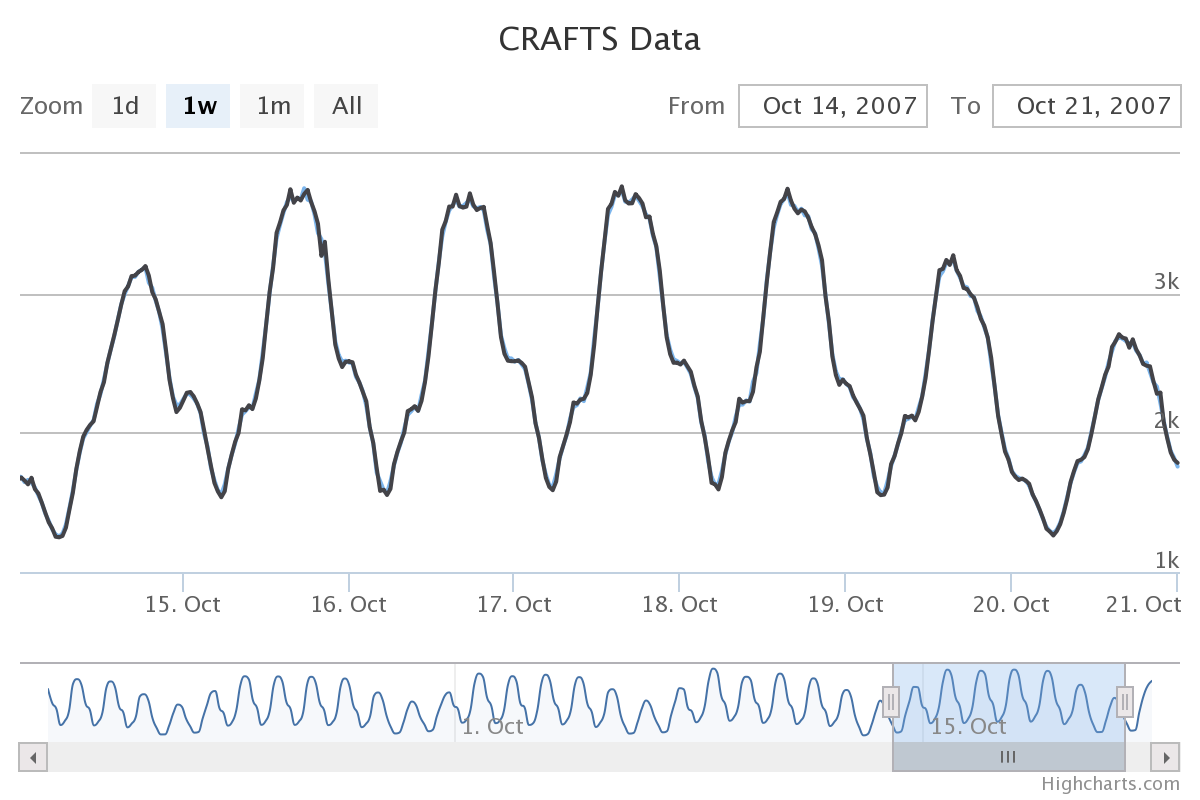
\includegraphics[width=\textwidth]{results/graphs/smoothing_baseline.png}
\caption{Exponential smoothing prediction results for the baseline workload}
\label{fig:smoothing_b}
\end{figure}

\begin{table}[H]
\centering
\begin{tabular}{| l | l | l | l | l |}
\hline
Type & \multicolumn{2}{c |}{Regular} & \multicolumn{2}{c |}{Anomalous} \\ \hline
 & RMSD & Percent & RMSD & Percent \\ \hline
Under & 42 & 53.1\% & 31 & 72.7\% \\ \hline
Over & 48 & 46.9\% & 22 & 27.3\% \\ \hline
Total & 45 & & 29 & \\ \hline
\end{tabular}
\caption{Exponential smoothing predictor results for the training outage workload}
\end{table}

\begin{figure}[H]
\centering
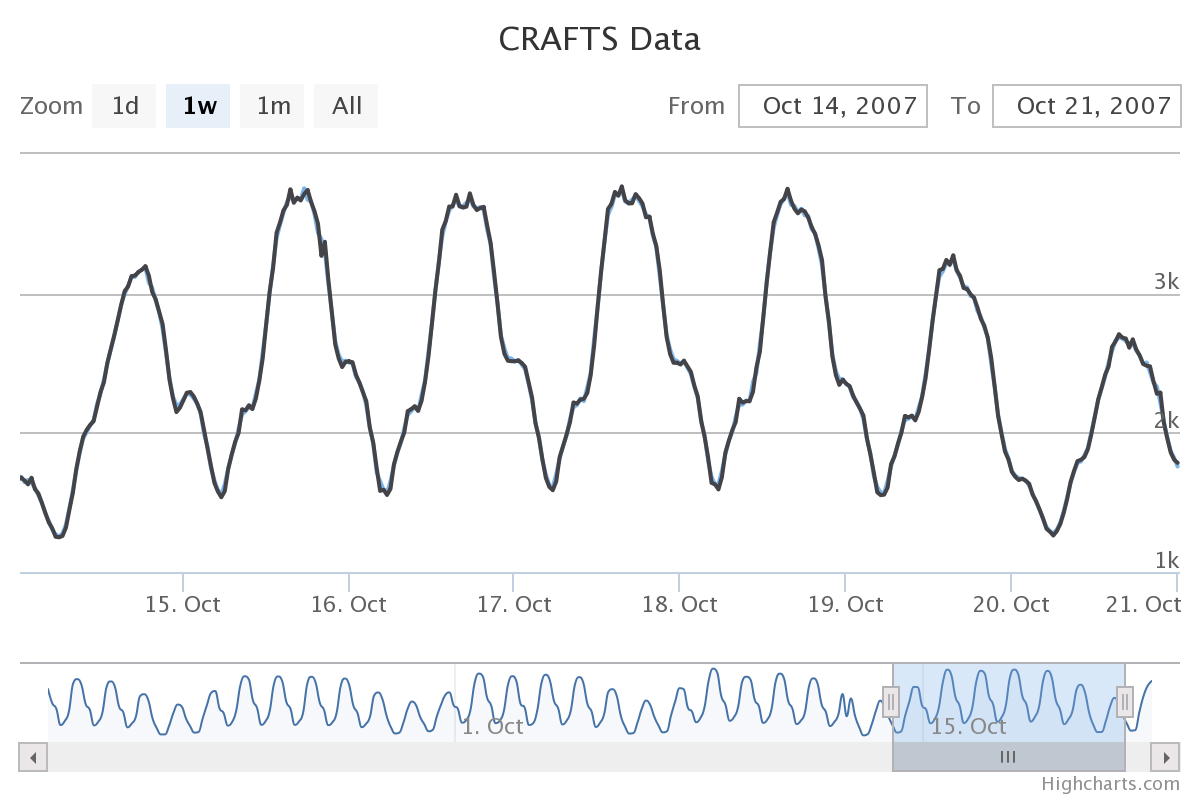
\includegraphics[width=\textwidth]{results/graphs/smoothing_training_outage.png}
\caption{Exponential smoothing prediction results for the training outage workload}
\label{fig:smoothing_to}
\end{figure}

\begin{table}[H]
\centering
\begin{tabular}{| l | l | l | l | l |}
\hline
Type & \multicolumn{2}{c |}{Regular} & \multicolumn{2}{c |}{Anomalous} \\ \hline
 & RMSD & Percent & RMSD & Percent \\ \hline
Under & 165 & 53.0\% & 1216 & 81.8\% \\ \hline
Over & 159 & 47.0\% & 3068 & 18.2\% \\ \hline
Total & 162 & & 1709 & \\ \hline
\end{tabular}
\caption{Exponential smoothing predictor results for the horizon outage workload}
\end{table}

\begin{figure}[H]
\centering
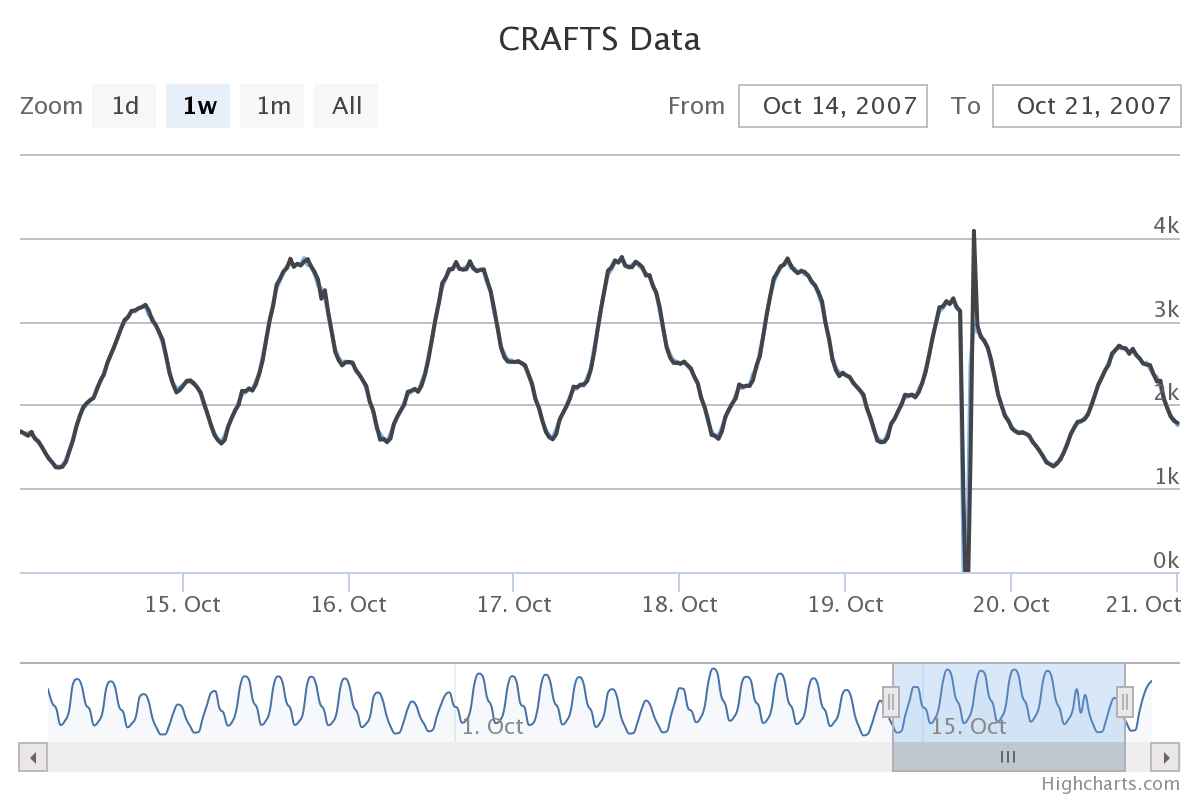
\includegraphics[width=\textwidth]{results/graphs/smoothing_horizon_outage.png}
\caption{Exponential smoothing prediction results for the horizon outage workload}
\label{fig:smoothing_ho}
\end{figure}

\begin{table}[H]
\centering
\begin{tabular}{| l | l | l | l | l |}
\hline
Type & \multicolumn{2}{c |}{Regular} & \multicolumn{2}{c |}{Anomalous} \\ \hline
 & RMSD & Percent & RMSD & Percent \\ \hline
Under & 42 & 53.2\% & 0 & 0.0\% \\ \hline
Over & 48 & 46.8\% & 16 & 100.0\% \\ \hline
Total & 45 & & 16 & \\ \hline
\end{tabular}
\caption{Exponential smoothing predictor results for the training spike workload}
\end{table}

\begin{figure}[H]
\centering
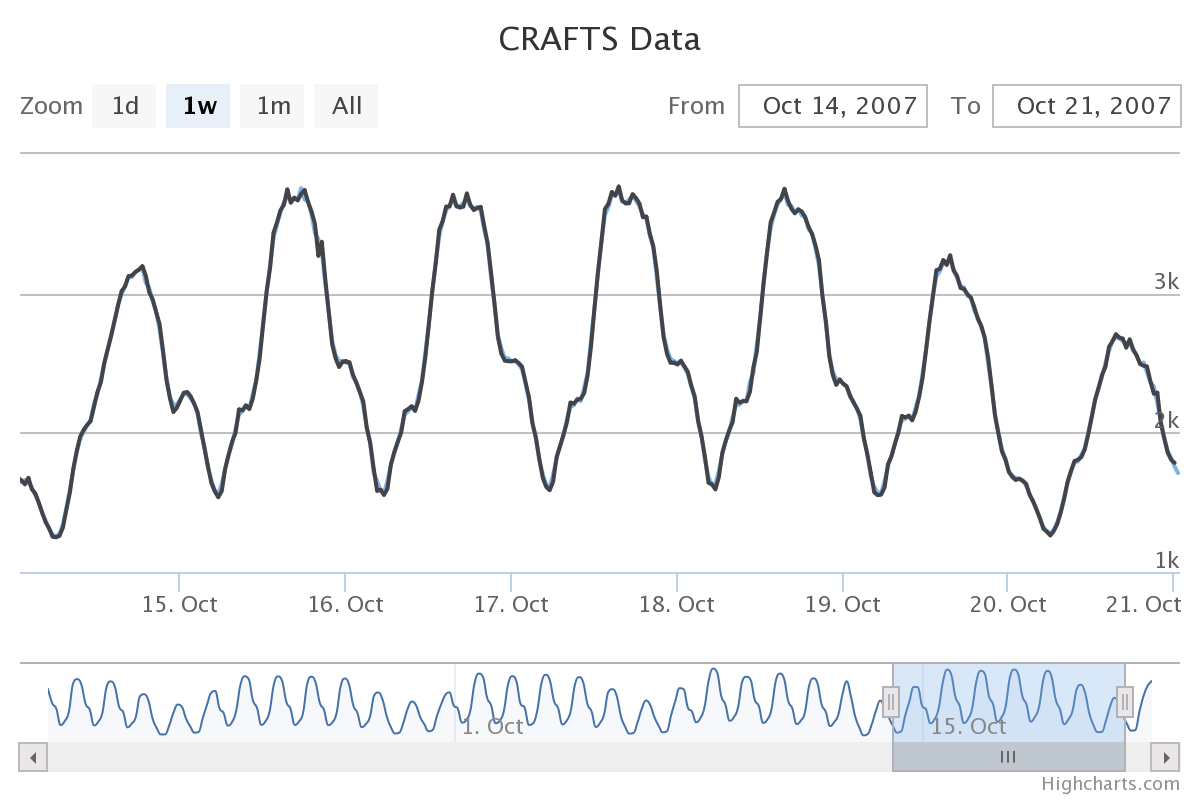
\includegraphics[width=\textwidth]{results/graphs/smoothing_training_spike.png}
\caption{Exponential smoothing prediction results for the training spike workload}
\label{fig:smoothing_ts}
\end{figure}

\begin{table}[H]
\centering
\begin{tabular}{| l | l | l | l | l |}
\hline
Type & \multicolumn{2}{c |}{Regular} & \multicolumn{2}{c |}{Anomalous} \\ \hline
 & RMSD & Percent & RMSD & Percent \\ \hline
Under & 129 & 53.2\% & 3036 & 100.0\% \\ \hline
Over & 277 & 46.8\% & 0 & 0.0\% \\ \hline
Total & 212 & & 3036 & \\ \hline
\end{tabular}
\caption{Exponential smoothing predictor results for the horizon spike workload}
\end{table}

\begin{figure}[H]
\centering
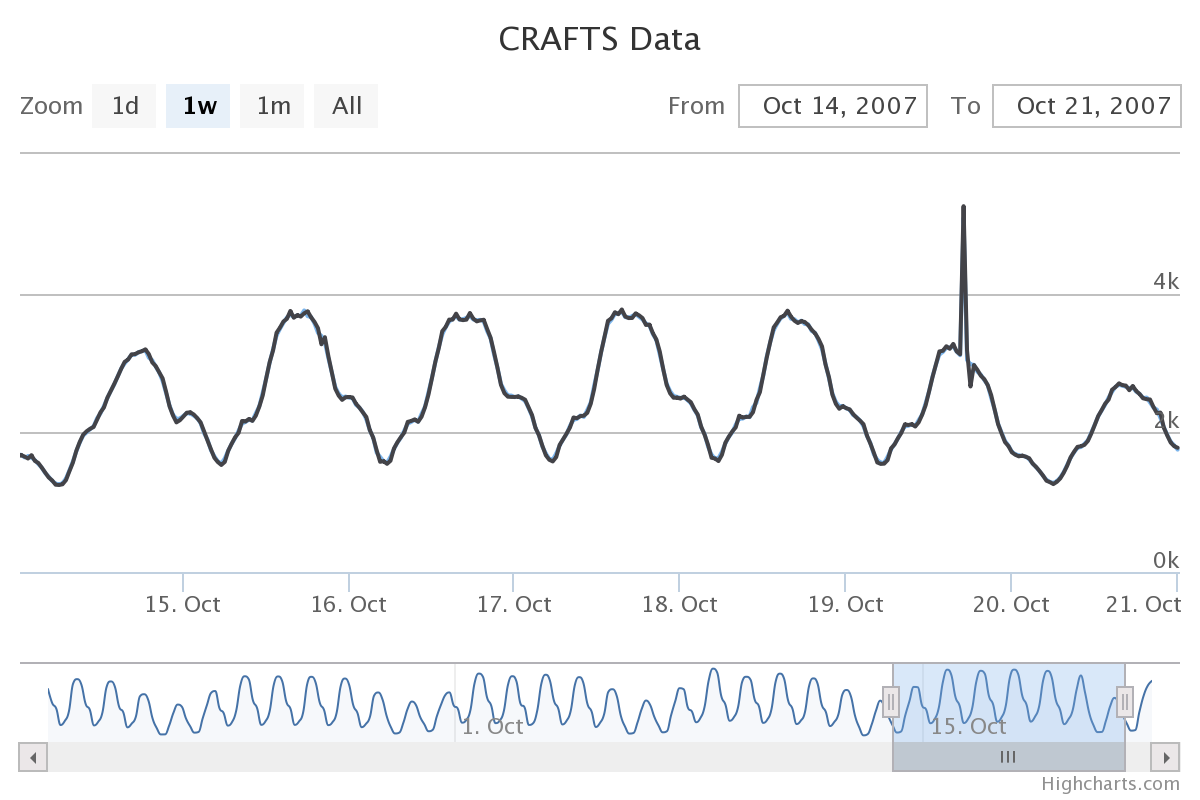
\includegraphics[width=\textwidth]{results/graphs/smoothing_horizon_spike.png}
\caption{Exponential smoothing prediction results for the horizon spike workload}
\label{fig:smoothing_hs}
\end{figure}